\documentclass[10pt,a4paper,twocolumn]{article}

\usepackage[margin=0.75in]{geometry}
\usepackage{graphicx}
\usepackage{booktabs}
\usepackage{subcaption}
\usepackage{hyperref}

\title{A Short Two-Column Article Demo}
\author{CSE200}
\date{}

\begin{document}

\maketitle

\section{Why a Separate File?}

{\raggedright
Package note: this document requests two columns with the \texttt{twocolumn}
class option. It also uses \texttt{graphicx}, \texttt{subcaption},
\texttt{booktabs}, and \texttt{hyperref}.
\par}

A real two-column document behaves differently from a small two-column block
inside a single-column article. Paragraphs flow from the left column to the
right column, floats may move differently, and wide figures need special
environments.

\section{Normal Column-Width Figure}

Package note: the image command \verb|\includegraphics| needs
\verb|\usepackage{graphicx}|.

\begin{figure}[ht]
    \centering
    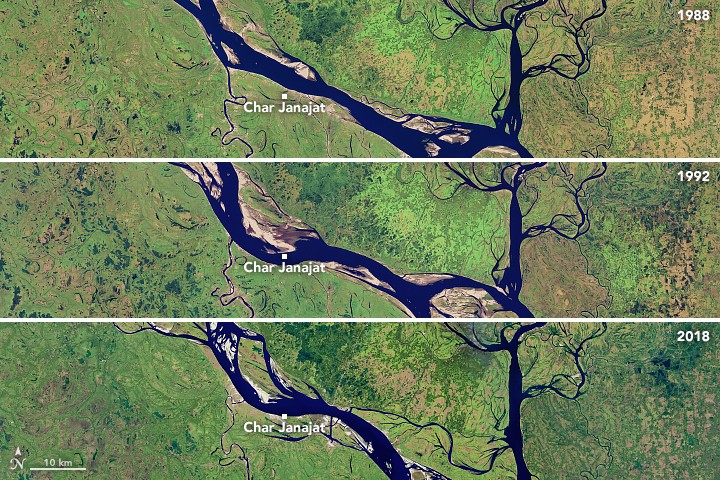
\includegraphics[width=\linewidth]{images/padma_river.jpg}
    \caption{A normal figure occupies one column.}
    \label{fig:column-padma}
\end{figure}

Figure~\ref{fig:column-padma} uses \verb|width=\linewidth|. In a two-column
document, \verb|\linewidth| means the width of one column.

\section{A Wide Figure}

Package note: \texttt{figure*} is built into two-column LaTeX output.
The subfigures inside this example need \verb|\usepackage{subcaption}|.

\begin{figure*}[t]
    \centering
    \begin{subfigure}{0.31\textwidth}
        \centering
        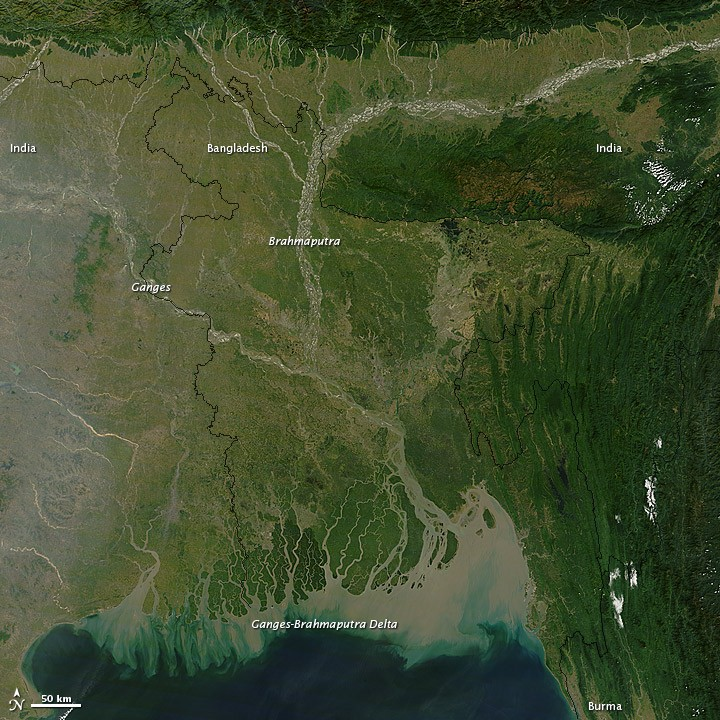
\includegraphics[width=\linewidth]{images/bangladesh_satellite.jpg}
        \caption{Bangladesh}
    \end{subfigure}
    \hfill
    \begin{subfigure}{0.31\textwidth}
        \centering
        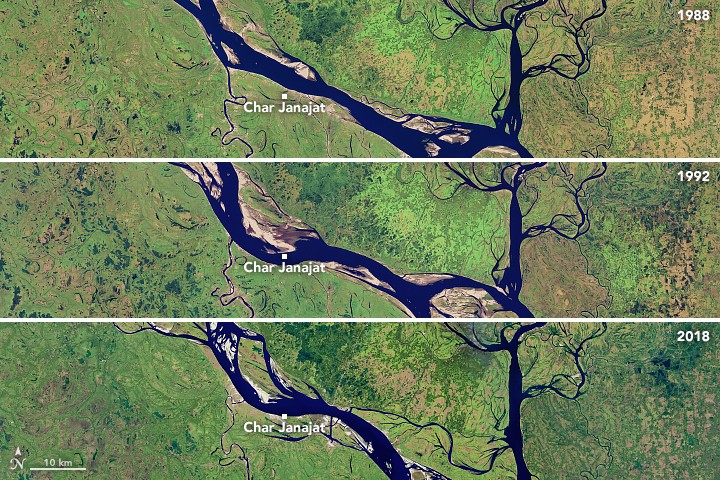
\includegraphics[width=\linewidth]{images/padma_river.jpg}
        \caption{Padma River}
    \end{subfigure}
    \hfill
    \begin{subfigure}{0.31\textwidth}
        \centering
        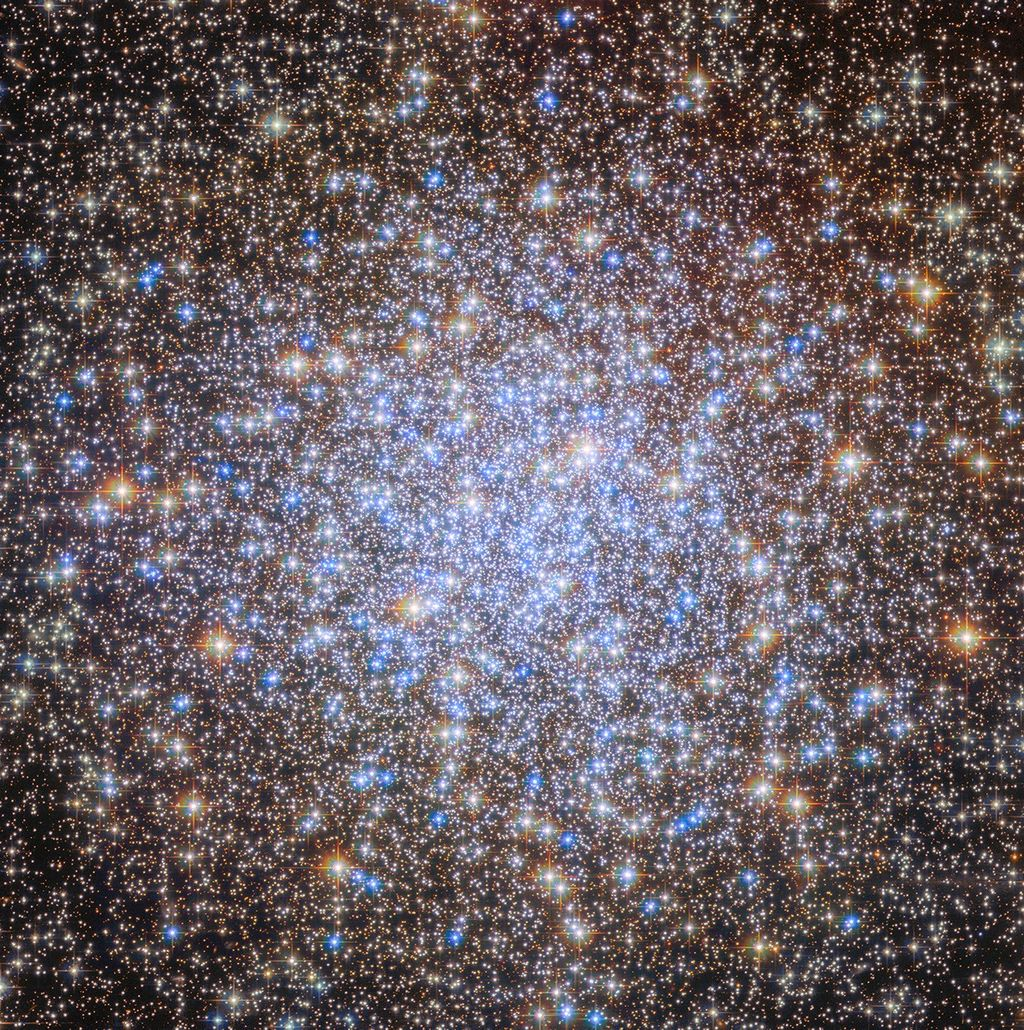
\includegraphics[width=\linewidth]{images/hubble_cluster.jpg}
        \caption{Hubble image}
    \end{subfigure}
    \caption{A wide figure spanning both columns with \texttt{figure*}.}
    \label{fig:wide-comparison}
\end{figure*}

Wide figures such as Figure~\ref{fig:wide-comparison} usually appear at the
top of a page. In two-column writing, this behavior is normal.

\section{Two-Column Table}

{\raggedright
Package note: ordinary \texttt{tabular} is built in. The rule commands
\verb|\toprule|, \verb|\midrule|, and \verb|\bottomrule| need
\texttt{booktabs}.
\par}

\begin{table}[ht]
    \centering
    \begin{tabular}{ll}
        \toprule
        Concept & Command \\
        \midrule
        One-column figure & \texttt{figure} \\
        Two-column figure & \texttt{figure*} \\
        Column width & \verb|\linewidth| \\
        Page text width & \verb|\textwidth| \\
        \bottomrule
    \end{tabular}
    \caption{Width commands in two-column documents.}
    \label{tab:two-column-widths}
\end{table}

\section{Citation in Two Columns}

Package note: this example uses plain BibTeX, so no citation package is needed.
It uses the built-in \verb|\cite| command with \verb|\bibliographystyle| and
\verb|\bibliography|.

{\raggedright
Citations work the same way in a two-column article. For example, attention
models can be cited with plain BibTeX~\cite{vaswani2017attention}, and residual
networks can be cited the same way~\cite{he2016deep}.
\par}

\bibliographystyle{plain}
\bibliography{references}

\end{document}
